% ========================================================================== %
\section{Validation on simulations} \label{sec:simu}

In order to ensure that \panco\ is able to recover accurate pressure profile measurements, we test it on simulated inputs.
In this section, we detail this validation process, from the creation of the dataset to the results produces by \panco.
For reproducibility purposes, the datasets created and used for this analysis are made public with the software.

% -------------------------------------------------------------------------- %
\subsection{Sample selection}

The goal of the validation is to ensure that \panco\ is able to recover accurate pressure profiles from different types of data.
To that end, we seek to create realistic synthetic cluster maps from three instruments: the \textit{Planck} satellite, the South Pole Telescope (SPT), and the NIKA2 camera at the IRAM 30 m telescope.
The choice of these three instruments is motivated by their vastly different angular resolutions: the Compton$-y$ maps built from \textit{Planck} and SPT data have angular resolutions (expressed as the full width at half maximum, or FWHM) of 10 and 1.25 arcmin, respectively \citep{planck_collaboration_planck_2016, bleem_cmbksz_2022}, and the beam of the NIKA2 camera 150 GHz band -- used for tSZ mapping -- has an FWHM of 18 arcsec \citep{perotto_calibration_2020}.

We choose to create SZ maps for three clusters, labeled (C1, C2, C3), covering different regions of the mass-redshift plane:
\begin{alignat}{2}
    \nonumber {\rm C1}:\; & z=0.05,\ & M_{500} = 9 \times 10^{14} \ M_\odot ;\\
    \nonumber {\rm C2}:\; & z=0.5,\  & M_{500} = 6 \times 10^{14} \ M_\odot ;\\
              {\rm C3}:\; & z=1,\    & M_{500} = 3 \times 10^{14} \ M_\odot,
    \label{eq:valid:clusters}
\end{alignat}
These mock clusters are shown as black stars in figure~\ref{fig:valid:sample}.
The top panel shows their positions in the mass-redshift plane, indicating that C1, C2 and C3 are realistic detections for the \textit{Planck}, SPT, and ACT tSZ surveys, respectively.
Tbe bottom panel of figure~\ref{fig:valid:sample} places the clusters in the angular diameter-redshift plane, showing that C1 can be resolved in \textit{Planck}, SPT, and NIKA2 tSZ maps, while C2 and C3 are too small to be resolved by \textit{Planck}.

\begin{figure}[tp]
    \centering
    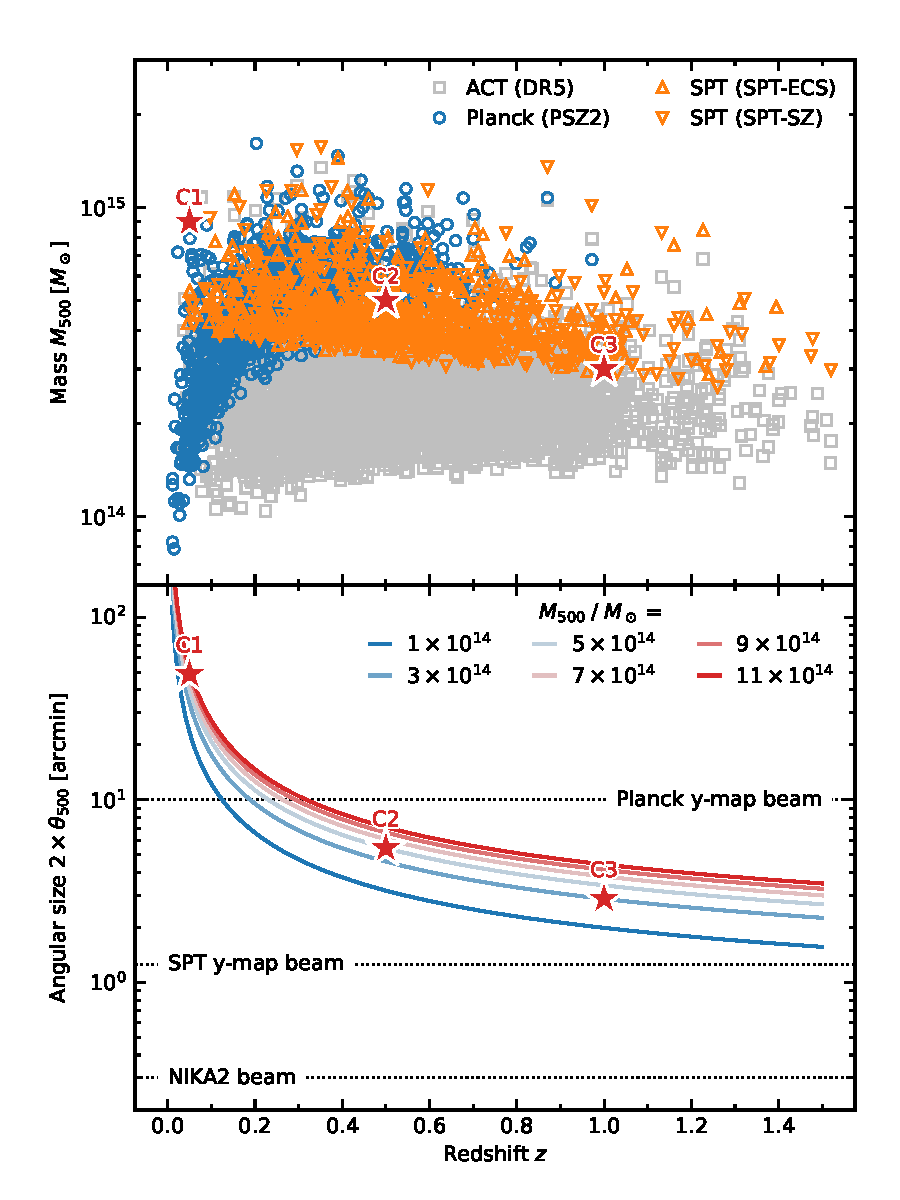
\includegraphics[width=\linewidth]{Figures/validation_sample.pdf}
    \caption{
        Validation cluster sample (black stars) in the mass-redshift plane (\textit{top panel}) and in the angular size-redshift plane (\textit{bottom panel}).
        For illustration, the top panel includes clusters detected in recent tSZ surveys: \textit{Planck} \citep{planck_collaboration_planck_2016-2}, ACT \citep{hilton_atacama_2021}, and SPT \citep{bleem_sptpol_2020,bleem_galaxy_2015}.
        Note that the redshift axis is truncated to $z<1.6$, therefore not showing all clusters in these samples.
        Colored lines in the bottom panel show the evolution of the angular $2\times\theta_{500}$ with redshift for clusters of different masses.
        The angular resolutions of the \textit{Planck} and SPT $y-$maps, as well as that of the NIKA2 camera at 150~GHz, are represented as dotted horizontal lines.
    }
    \label{fig:valid:sample}
\end{figure}

% -------------------------------------------------------------------------- %
\subsection{Data generation}

We create mock maps for the three clusters by forward modeling their tSZ signal.
We assume that each cluster has a pressure profile that follows the universal profile of \aten, scaled with its mass and redshift.
This pressure distribution is integrated along the line of sight to obtain a Compton$-y$ map.
This map is then projected on a flat-sky grid and convolved with a Gaussian filter to account for instrumental filtering, and added to a random noise realization.

As discussed previously, and illustrated in the bottom panel of figure~\ref{fig:valid:sample}, the angular size of each cluster is very different, and the mapping of their tSZ signal is very different for all instruments considered.
We therefore create different sets of maps for the three clusters.
For C1, the most extended cluster, we create mock \textit{Planck} and SPT maps.
For C2, our intermediate case, we create SPT and NIKA2 mock maps.
Finally, for C3, the smallest cluster in our sample, we only create mock NIKA2 data.
The characteristics of the maps are designed to mimic know cluster observations by the three instruments, and summarized in table~\ref{tab:simu:map_props}.
The generated maps are shown in figure~\ref{fig:valid:sample}.

\paragraph{Planck-like data}  % ............................................ %
Our mock \textit{Planck} dataset is designed to emulate the \textit{Planck} Compton$-y$ map of \citet{planck_collaboration_planck_2016}.
The original data products for this map are in \texttt{healpix} format, which \panco\ cannot process, as it relies on the flat-sky approximation.
We therefore create maps of $(5\degree \times 5\degree)$ patches of the sky using a gnomonic projection, with a pixel size of $2'$, and a Gaussian PSF of ${\rm FWHM} = 10'$.
The noise in these maps is white and has an homogeneous distribution, with an RMS taken from the left panel of figure~13 in \citet{planck_collaboration_planck_2016}.
\todo{filtering?}
\todo{correlated noise?}

\paragraph{SPT-like data}  % ............................................... %
Our SPT-like maps mimic the plublicly available $y-$maps released by the SPT collaboration \citep{bleem_cmbksz_2022}.
We use the same projection as their flat-sky maps, \ie\ a Sanson-Flamsteed projection with $15''$ pixels, on a $(1\degree \times 1\degree)$ patch of the sky.
The resolution of the map is Gaussian with ${\rm FWHM} = 1.25'$.
We inject a white noise realization, the amplitude of which is evaluated by computing the RMS of the map in a $(5\degree \times 5\degree)$ patch of the sky, taking care of masking sources.
\todo{filtering?}
\todo{correlated noise?}

\paragraph{NIKA2-like data}  % ............................................. %
Our NIKA2-like data imitates the NIKA2 150~GHz sky maps obtained by the NIKA2 SZ Large Program \citep{mayet_cluster_2020, perotto_nika2_2021}.
In particular, we use the data products publicly released in \citet{keruzore_exploiting_2020}.
We create a gnomonic projection of a $(6.5' \times 6.5')$ patch of the sky with $3''$ pixels.
The angular resolution of the map is Gaussian with ${\rm FWHM} = 18''$, and we also take into account filtering of angular scales due to data processing via the transfer function of \citet{keruzore_exploiting_2020}.
The noise in these NIKA2 maps is considered white and isotropic, but not homogeneous, as the NIKA2 on-the-fly scanning strategy used for obsevations of the NIKA2 SZ Large Program creates a variation in the noise level of the maps depending on the distance from the pointing coordinates.
To accurately take into account this effect, we use the noise RMS map of \citet{keruzore_exploiting_2020}, which we multiply by a scalar value to account for different exposure times.

\begin{table*}[t]
    \centering
    \begin{tabular}{l c c c c c c}
        \toprule
        Instrument & Clusters & Map size & Pixel size & FWHM & Filtering & Noise \\
        \midrule
        \multirow{2}{*}{\textit{Planck}} & \multirow{2}{*}{C1} & \multirow{2}{*}{$5\degree$} & \multirow{2}{*}{$2'$} & \multirow{2}{*}{$10'$} & \multirow{2}{*}{--} & White, Homogeneous \\
            & & & & & & RMS=$4.12 \times 10^{-6} \; [y]$ \\
        \midrule
        \multirow{2}{*}{SPT} & \multirow{2}{*}{C1, C2} & \multirow{2}{*}{$1\degree$} & \multirow{2}{*}{$15''$} & \multirow{2}{*}{$1.25'$} & -- & White, Homogeneous, \\
            & & & & & & RMS=$9.78 \times 10^{-6} \; [y]$ \\
        \midrule
        \multirow{2}{*}{NIKA2} & \multirow{2}{*}{C2, C3} & \multirow{2}{*}{$6.5'$} & \multirow{2}{*}{$3''$} & \multirow{2}{*}{$18''$} & NIKA2-like & White, isotropic \\
                               & & & & & transfer function & NIKA2-like RMS \\
        \bottomrule
    \end{tabular}
    \caption{\normalfont
        Properties of simulated maps emulating cutouts of the \textit{Planck} \citep{planck_collaboration_planck_2016} and SPT \citep{bleem_cmbksz_2022} $y-$maps, and NIKA2 cluster observations \citep{keruzore_exploiting_2020}.
    }
    \label{tab:simu:map_props}
\end{table*}

\begin{figure*}[t]
    \centering
    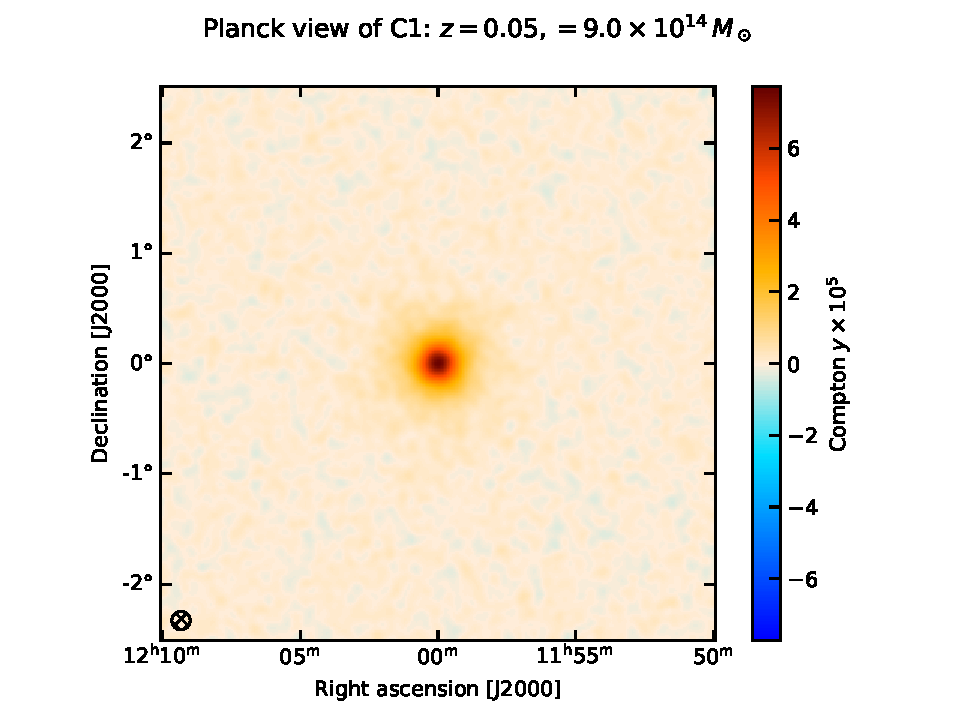
\includegraphics[page=1, width=0.49\linewidth, trim={1cm 0cm 1cm 1cm}, clip]{Figures/sim_maps.pdf}
    \includegraphics[page=2, width=0.49\linewidth, trim={1cm 0cm 1cm 1cm}, clip]{Figures/sim_maps.pdf}
    \includegraphics[page=3, width=0.49\linewidth, trim={1cm 0cm 1cm 1cm}, clip]{Figures/sim_maps.pdf}
    \includegraphics[page=4, width=0.49\linewidth, trim={1cm 0cm 1cm 1cm}, clip]{Figures/sim_maps.pdf}
    \includegraphics[page=5, width=0.49\linewidth, trim={1cm 0cm 1cm 1cm}, clip]{Figures/sim_maps.pdf}
    \caption{%
        Simulated maps of the three validation clusters.
        \textbf{Top:} C1 seen by \textit{Planck} (\textit{left}) and SPT (\textit{right});
        \textbf{Middle:} C2 seen by SPT (\textit{left}) and NIKA2 (\textit{right});
        \textbf{Bottom:} C3 seen by NIKA2.
        Map properties are summarized in table~\ref{tab:simu:map_props}, and the cluster properties in eq.~(\ref{eq:valid:clusters}).
        Each map is smoothed with a Gaussian filter with $\sigma = 1 \; {\rm pixel}$ for displaying purposes.
        The FWHM of the angular resolution of each map is shown as a hatched circle in its bottom left.
    }
    \label{fig:valid:maps}
\end{figure*}

% -------------------------------------------------------------------------- %
\subsection{Pressure profile fitting}

% -------------------------------------------------------------------------- %
\subsection{Results} \label{sec:simu:results}

\begin{figure*}[t]
    \centering
    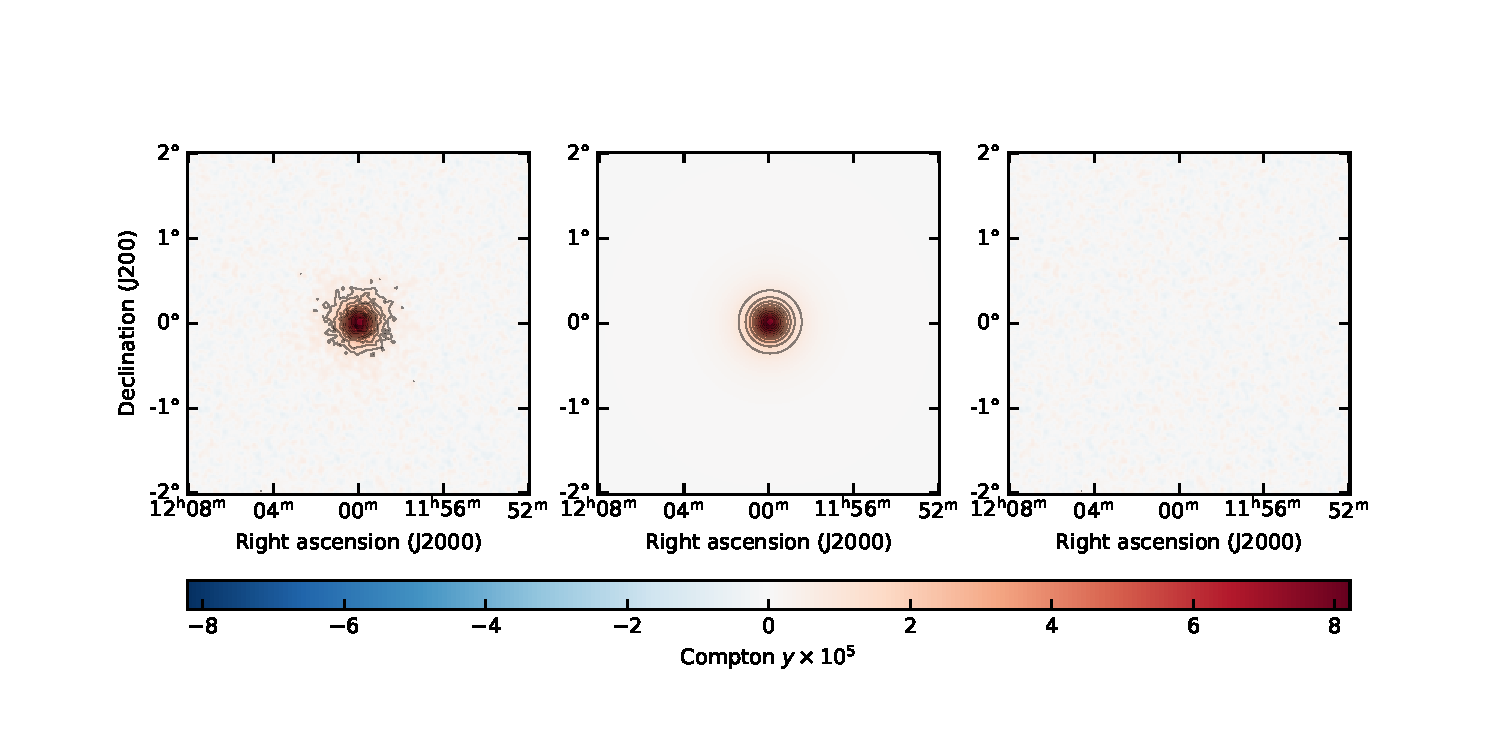
\includegraphics[width=\linewidth, trim={0 1cm 0 2cm}, clip]{Figures/C1_planck_dmr_2d.pdf}
    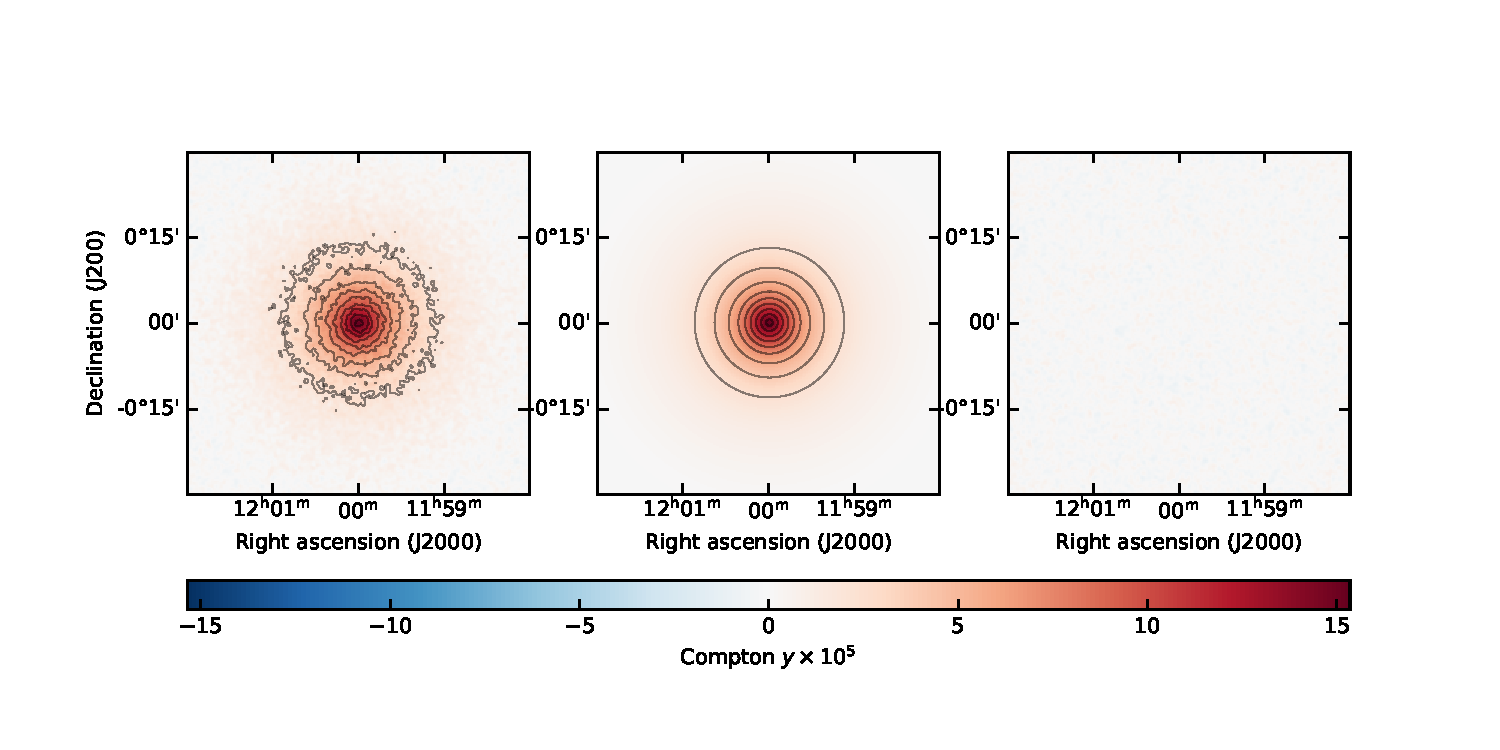
\includegraphics[width=\linewidth, trim={0 1cm 0 2cm}, clip]{Figures/C1_spt_dmr_2d.pdf}
    \caption{}
    \label{fig:}
\end{figure*}
